\documentclass[11pt]{article}
\usepackage{lscape}
\usepackage[utf8]{inputenc}
\usepackage[T1]{fontenc}
\usepackage{graphicx}
\usepackage{grffile}
\usepackage{longtable}
\usepackage{graphicx}
\usepackage{wrapfig}
\usepackage{rotating}
\usepackage{csquotes}
\usepackage[normalem]{ulem}
\usepackage{amsmath}
\usepackage{textcomp}
\usepackage{amssymb}
\usepackage{capt-of}
\usepackage{hyperref}
\usepackage{indentfirst}
\usepackage[T2A]{fontenc}
\usepackage[a4paper,left=3cm,top=2cm,right=1.5cm,bottom=2cm,marginparsep=7pt,marginparwidth=.6in]{geometry}
\usepackage{cmap}
\usepackage[russian]{babel}
\usepackage{fancyhdr}
\usepackage{xcolor}
\usepackage{minted}
\usepackage{color}
\usepackage{listings}
\usepackage{url}
\urlstyle{same}
\newcommand\purl[1]{\protect\url{#1}}
\author{АВТОР}
\date{\today}
\title{}
\hypersetup{
	pdfauthor={АВТОР},
	pdftitle={},
	pdfkeywords={},
	pdfsubject={},
	pdfcreator={Emacs 26.1 (Org mode 9.1.9)}, 
	pdflang={Russian}}
\setlength{\parindent}{5ex}
\setlength{\parskip}{1em}
\begin{document}
\thispagestyle{empty}
\begin{center}
\textbf{Национальный Исследовательский Университет ИТМО}\\
\textbf{Факультет Программной Инженерии и Компьютерной Техники}\\
\end{center}
\vspace{2em}
\begin{center}

\includegraphics[width=120px]{../../../itmo-logo.png}
\end{center}
\LARGE
\vspace{5em}
\begin{center}
\textbf{Вариант № 86006}\\
\textbf{Лабораторная работа № 3}\\
\Large
\textbf{по дисциплине}\\
\LARGE
\textbf{\emph{'Программирование'}}\\
\end{center}
\vspace{11em}
\large
\begin{flushright}
\textbf{Выполнил:}\\
\textbf{Студент группы P3113}\\
\textbf{\emph{Куперштейн Дмитрий;} : 269359}\\
\textbf{Преподаватель:}\\
\textbf{\emph{ПИСЬМАК АЛЕКСЕЙ ЕВГЕНЬЕВИЧ}}\\
\end{flushright}
\vspace{4em}
\large
\begin{center}
\textbf{Санкт-Петербург 2019 г.}
\end{center}
\pagebreak{}
\setcounter{tocdepth}{2}
\tableofcontents
\vspace{2em}
\pagebreak
\large
\section{Задание}
Описание предметной области, по которой должна быть построена объектная модель (для варианта 86006):
\begin{displayquote}
	"Страсть как забавно, -- подумала она. -- Вот уж удивится моя сестра!" Оглядевшись вокруг, она заметила плывшие рядом поднос для пирожков и шкатулку Муми-мамы. После недолгого раздумья (хотя на подносе еще оставалось несколько пирожков) она выбрала шкатулку и залезла туда.
\end{displayquote}
Программа должна удовлетворять следующим требованиям:
\begin{enumerate}
	\item Доработанная модель должна соответствовать принципам SOLID.
	\item Программа должна содержать как минимум два интерфейса и один абстрактный класс (номенклатура должна быть согласована с преподавателем).
	\item В разработанных классах должны быть переопределены методы \texttt{equals()},\texttt{ toString()} и \texttt{hashCode()}.
\pagebreak
\end{enumerate}
\section{Диаграмма классов объектной модели}
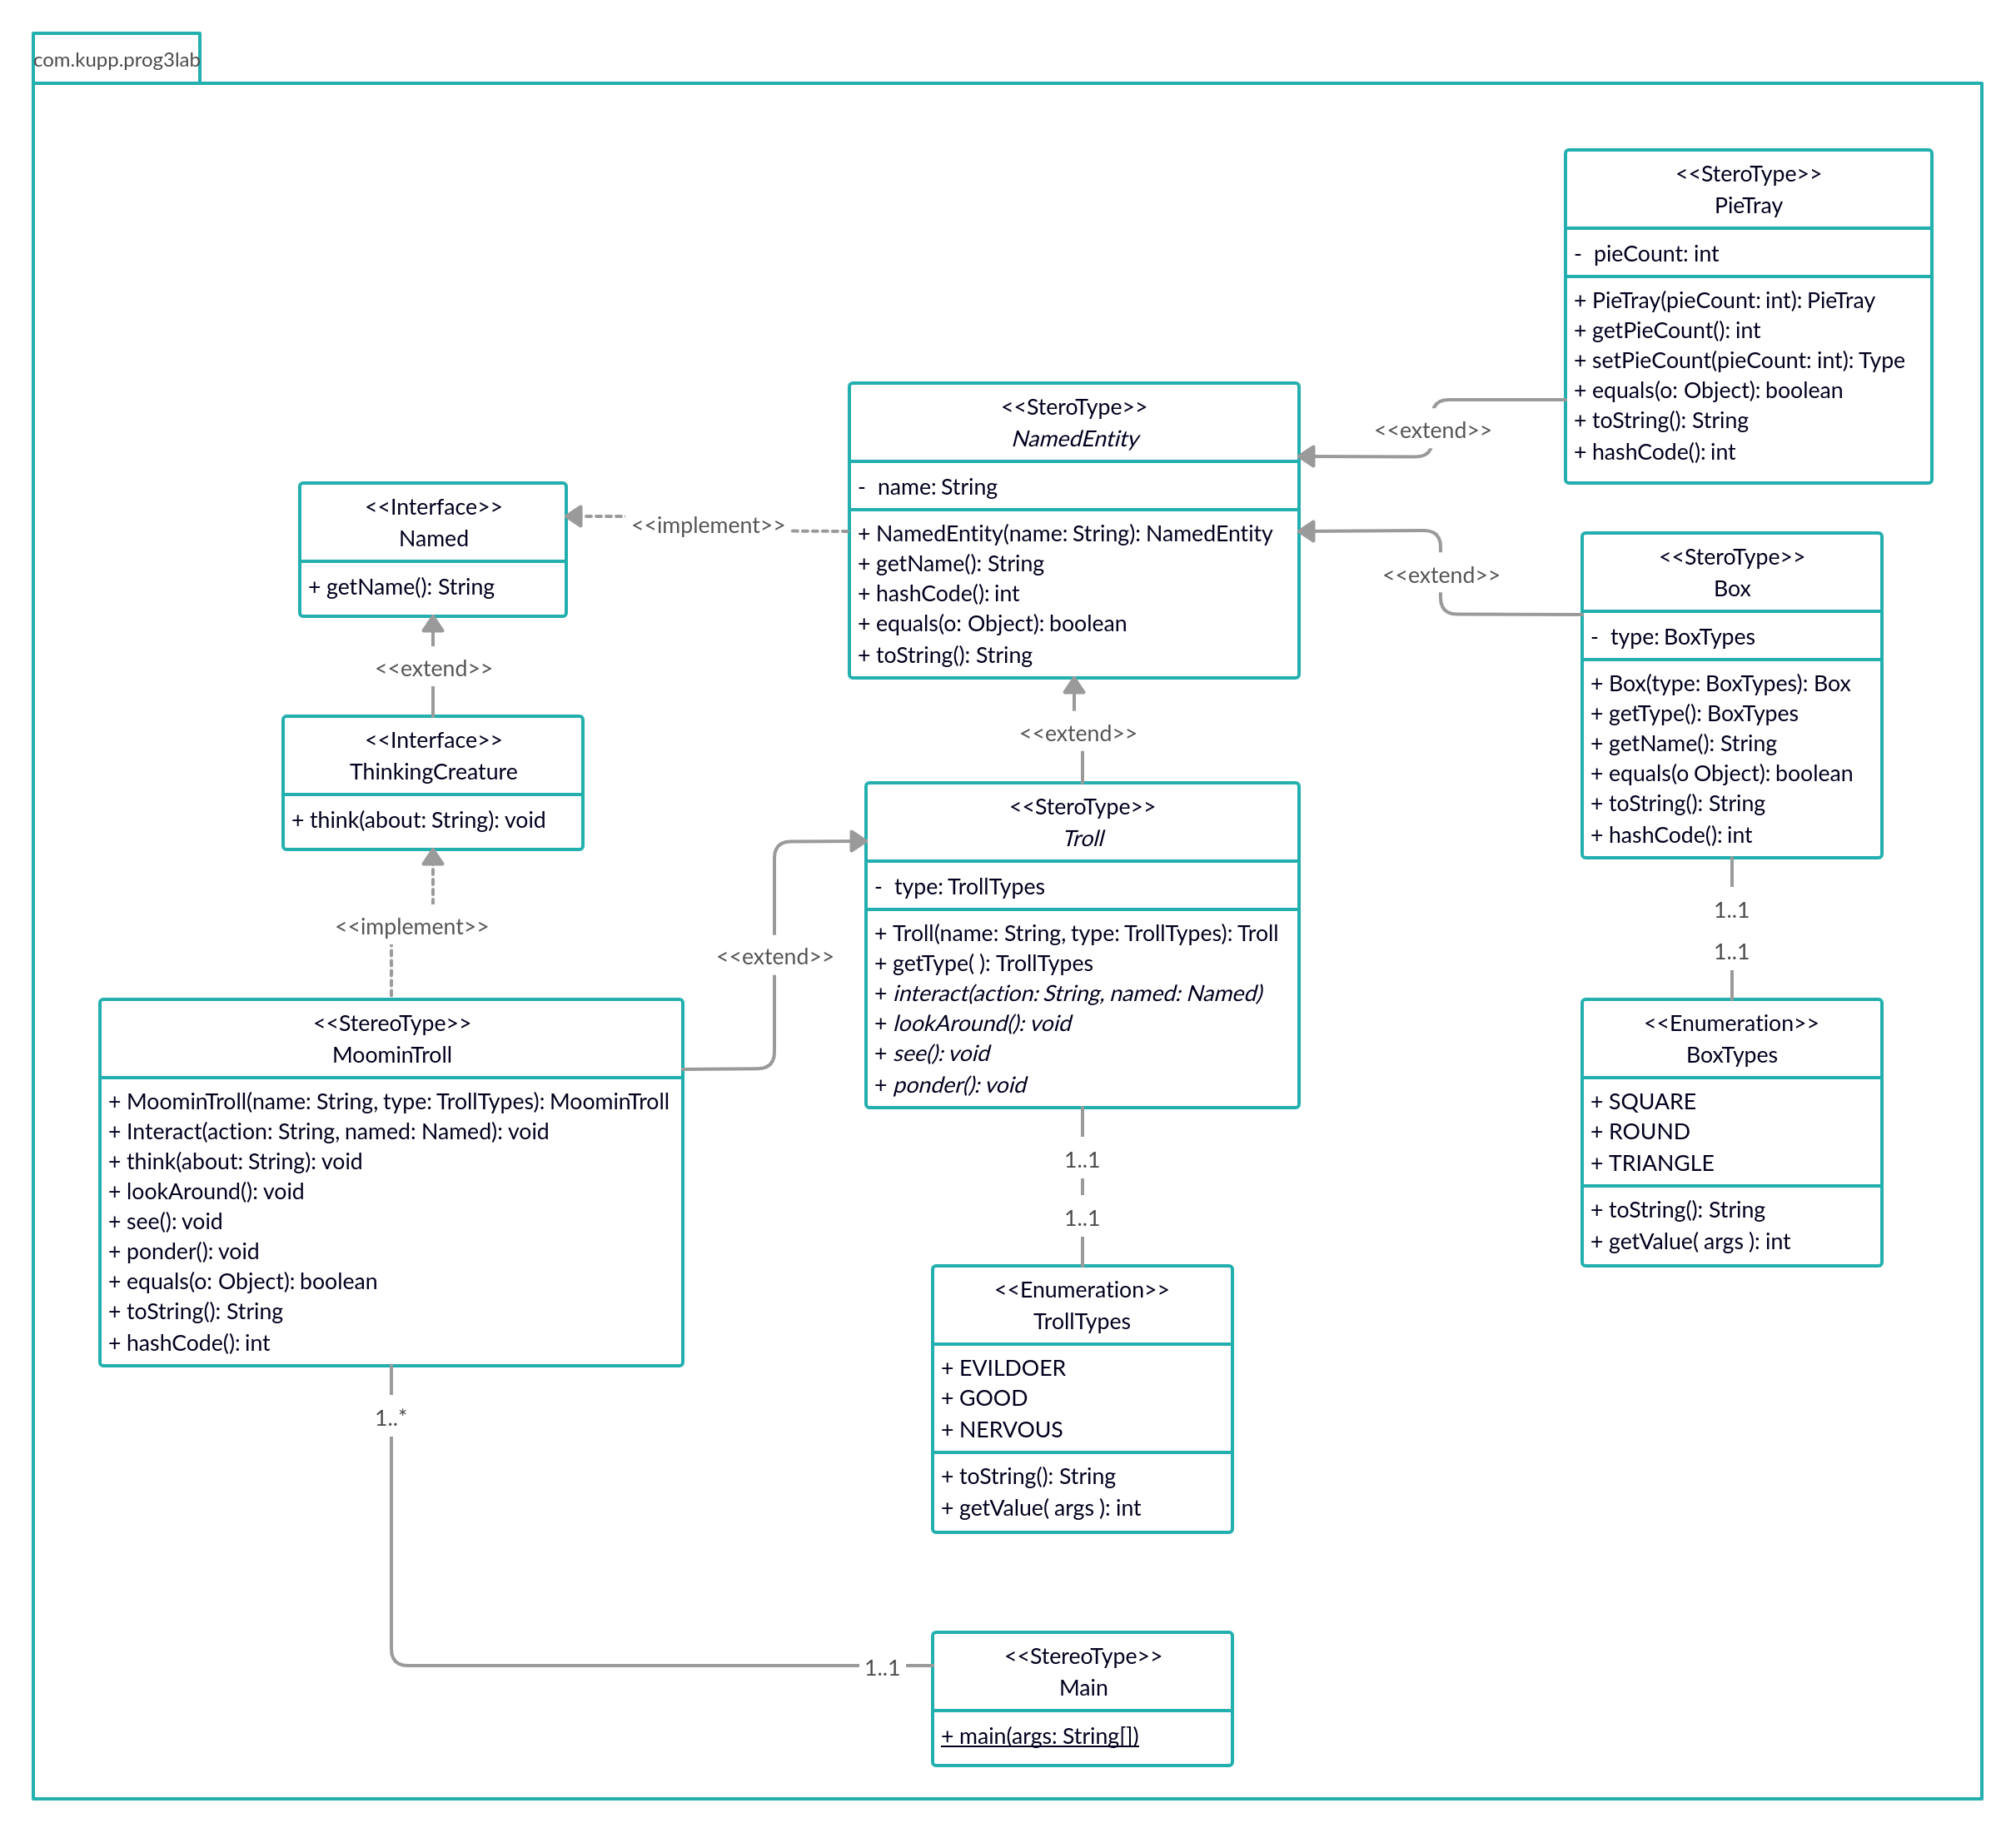
\includegraphics[width=470px]{../prog3lab class diagram.png}
\pagebreak
\section{Исходный код программы}
\small
\subsubsection{Main.java}
\inputminted{java}{../prog3lab/src/main/java/com/kupp/prog3lab/Main.java}
\subsubsection{Named.java}
\inputminted{java}{../prog3lab/src/main/java/com/kupp/prog3lab/Named.java}
\subsubsection{NamedEntity.java}
\inputminted{java}{../prog3lab/src/main/java/com/kupp/prog3lab/NamedEntity.java}
\subsubsection{ThinkingCreature.java}
\inputminted{java}{../prog3lab/src/main/java/com/kupp/prog3lab/ThinkingCreature.java}
\subsubsection{Troll.java}
\inputminted{java}{../prog3lab/src/main/java/com/kupp/prog3lab/Troll.java}
\subsubsection{MoominTroll.java}
\inputminted{java}{../prog3lab/src/main/java/com/kupp/prog3lab/MoominTroll.java}
\subsubsection{PieTray.java}
\inputminted{java}{../prog3lab/src/main/java/com/kupp/prog3lab/PieTray.java}
\subsubsection{Box.java}
\inputminted{java}{../prog3lab/src/main/java/com/kupp/prog3lab/Box.java}
\subsubsection{TrollTypes.java}
\inputminted{java}{../prog3lab/src/main/java/com/kupp/prog3lab/TrollTypes.java}
\subsubsection{BoxTypes.java}
\inputminted{java}{../prog3lab/src/main/java/com/kupp/prog3lab/BoxTypes.java}
\section{Результат работы программы}
\inputminted{text}{../out.txt}
\section{Вывод}
\large
В ходе этой лабораторной работы я поломал голову над реализацией абстрактной объектной модели по тексту, это оказалось непростой задачей для меня, так как пришлось достраивать модель текста для соответствия работы требованиям. Также я научился вписывать в enum в Java дополнительные методы.
\end{document}